\section{Grundlagen und Ansätze der Virtualisierung von Testumgebungen}

Laut Duden leitet sich das Adjektiv "`virtuell"' vom lateinischen "`virtus"' für "`Kraft, Tugend, Männlichkeit"' ab. Es bedeutet so viel wie "`von unwirklicher, scheinbarer, nicht tatsächlicher Form"'.

Innerhalb der Informatik kann man von zwei unterschiedlichen Arten der Virtuatlität sprechen. Zum einen gibt es den Bereich der "virtuellen Realität", bei der einem Menschen mit Hilfe einer in Echtzeit computergenerierten Umgebung das Gefühl vermittelt wird, sich in einer anderen Wirklichkeit zu befinden. Zum anderen gibt es eben den Bereich der Virtualisierung, bei dem es darum geht, einem Anwender (Mensch oder auch Programm) bestimmte Rahmenbedingungen vorzuspielen, die so eigentlich nicht existieren.

Ein einfaches Beispiel für Virtualisierung sind Hardware-Emulatoren. Hardware-Emulatoren gaukeln Software vor, mit einer Hardware zu interagieren, die so physisch gar nicht existiert. Dies wird z.B. verwendet, um alte Spiele von nicht mehr produzierten Spielekonsolen auf aktuellen Computern auszuführen oder auch um Apps für mobile Geräte wie Smartphones oder Tablets auf Desktoprechnern zu entwickeln oder zu testen, ohne diese Geräte wirklich vorzuhalten.

Ein weiteres Beispiel ist die Virtualisierung von Netzwerkressourcen. So können z.B. VLANs (Virtual Local Area Networks) verbundenen Geräten eine ganz andere Verkabelung vorgaukeln als sie physikalisch vorliegt, um so bestimmte Zugriffe zu erlauben oder zu sperren.

Der für diese Arbeit interessante Bereich der Virtualisierung ist das Bereitstellen virtueller Betriebsumgebungen. Eine Betriebsumgebung meint die Umgebung, die ein Programm für seine Ausführung benötigt. Dazu gehören vor allem bestimmte Hardware-Bauteile (Prozessoren, Arbeitsspeicher, Festplatten, Netzwerk-Adapter), ein Betriebssystem und eventuell zusätzliche Anwendungsprogramme, mit denen das Programm interagiert. Für gewöhnlich läuft eine solche Betriebsumgebung genau auf einem Rechner (z.B. Server oder Desktoprechner). Es gibt nun verschiedene Ansätze eine solche Betriebsumgebung zu virtualisieren, die sich hinsichtlich ihrer Implementierung und Funktionalität unterscheiden. Grundsätzlich unterscheidet man zwischen der Systemvirtualisierung mittels Hypervisor und der Betriebssystemvirtualisierung mittels OS-Containern. Auf diese Varianten soll nun im Näheren eingegangen werden, um so mögliche Kandidaten für die Virtualisierung von Testumgebungen gemäß der Problemstellung zu finden.

\begin{figure}[!ht]
  \begin{center}
    \includegraphics[width=8cm]{bilder/Einordnung_Virtualisierungstechnologien_für_virtuelle_Betriebsumgebungen.png}
    \caption{Einordnung Virtualisierungtechnologienen für virtuelle Betriebsumgebungen \citep{Hirschbach06}}
  \end{center}
\end{figure}

\subsection{Systemvirtualisierung mittels Hypervisor}

Als Hypervisor oder auch \ac{VMM} wird eine Software bezeichnet, die die physisch vorhandene Hardware abstrahiert und mehreren Gastbetriebssystemen zur Verfügung stellt. Dabei spielt es den Gastsystemen jeweils vor, dass sie auf einem eigenen vollständigen Rechner mit Prozessor, Arbeitsspeicher, Festplatte und sonstigen Geräten laufen. Ein solcher virtueller Rechner wird auch \ac{VM} genannt. Je nach tatsächlich vorhandener Hardware muss der \ac{VMM} dabei die Hardware für das Gastsystem emulieren, virtualisieren oder paravirtualisieren. Emulieren meint hierbei, das der \ac{VMM} dem Gastsystem eine Hardware anbietet, die garnicht existiert. Virtualisieren meint, dass er Zugriffe des Gastsystems auf die virtuelle Hardware entsprechend auf die physische Hardware übersetzt. Paravirtualisierung findet dann statt, wenn die physische Hardware selbst das Konzept der Virtualisierung versteht und die Zugriffe des Gastsystems zumindest teilweise selbst verarbeiten kann. Hierbei unterscheiden sich die unterschiedlichen Ansätze natürlich vorallem hinsichtlich ihrer Performance, da das Übersetzen der Zugriffe oder das komplette Emulieren einer Hardware aufwendiger ist, als direkt auf die Hardware zuzugreifen.

Robert P. Goldberg, der die Grundlagen des \ac{VMM} in den 70er Jahren wissenschaftlich erarbeitet hat, unterscheidet in seiner Doktorarbeit "`Architectural Principles for Virtual Computer Systems"' zwei Klassen des \ac{VMM} \citep[vgl.][S. 22 ff.]{Goldberg73}: Dem Typ I \ac{VMM} oder auch "`Bare Metal Hypervisor"' und dem Typ II \ac{VMM} oder auch "`Hosted Hypervisor"'. In den folgenden beiden Unterkapiteln sollen diese beiden Klassen und entsprechende Implementierungen näher beleuchtet werden.

Darauf folgt abschließend ein Unterkapitel zu den sogenannten Unikernels, einer relativ neuen Entwicklung innerhalb der Systemvirtualisierung mittels Hypervisor, die eine bestimmte Art von \acs{VM} beschreibt \citep[siehe Abstract]{MadMorAnd13}.

\subsubsection{Bare Metal Hypervisors}

Ein Bare Metal Hypervisor ist ein \ac{VMM}, der als eigenständiges Programm direkt auf echter physischer Hardware läuft und somit kein Betriebssystem auf dem Hostsystem benötigt.

\begin{figure}[!ht]
  \begin{center}
    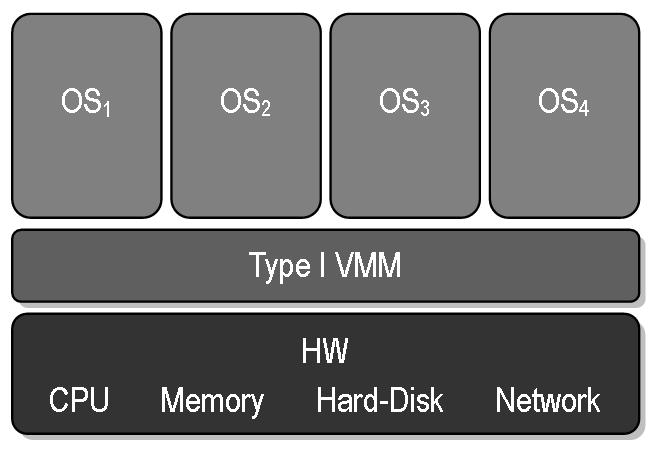
\includegraphics[width=8cm]{bilder/VMM-Type1.jpg}
    \caption{Virtual Machine Monitor Type I \citep{wiki:002}}
  \end{center}
\end{figure}

Durch diesen direkten Zugriff und das nicht notwendige Hostbetriebssystem gilt ein Bare Metal Hypervisor als ressourceneffizienter als ein Hosted Hypervisor. Größter Nachteil dieser Variante ist aber, dass sie mit mehr Installationsaufwand verbunden ist, da der Hypervisor selbst die passenden Gerätetreiber für die zugrundeliegende Hardware benötigt und man nicht auf Standardwerkzeuge wie zum Beispiel den Installationsmanagers eines Hostbetriebssystems zugreifen kann. Typische Vertreter dieser Hypervisor-Klasse sind zum Beispiel KVM und Citrix XenServer  \citep{wiki:004}.

Beim Open-Source-Produkt KVM (Kernel-based Virtual Machine) handelt es sich um eine Lösung, bei der ein normaler Linux-Kernel über ein spezielles Kernel-Modul für die grundsätzliche Virtualisierung (kvm.io) und ein weiteres prozessorspezifisches Kernel-Modul (kvm-intel.io oder kvm-amd.io) in die Lage versetzt wird, als Hypervisor zu arbeiten und Gastsysteme zu verwalten. KVM lässt sich damit grundsätzlich auf allen gängigen Linux Distributionen installieren. Oft wird deshalb vermutet, dass es sich nicht um einen reinen Bare Metal Hypervisor handelt, da er eben zusammen mit einem Betriebssystem installiert wird. Da es sich bei dem Kernel-Modul aber nicht um ein Anwendungsprogramm handelt, sondern um eine Erweiterung des eigentlichen Kernels, setzt diese Virtualisierungslösung direkt auf der darunterliegenden Hardware und nicht auf einem dazwischenliegenden Kernel auf \citep[Vgl.][]{kvm:001}.

\begin{figure}[!ht]
  \begin{center}
    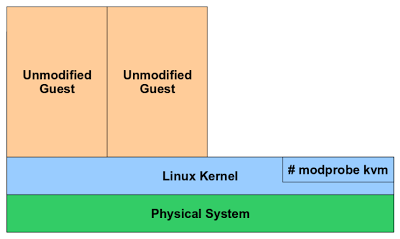
\includegraphics[width=8cm]{bilder/kvm.png}
    \caption{KVM Architektur \citep{kvm:002}}
  \end{center}
\end{figure}

So gibt es zum Beispiel die Linux Distribution Proxmox VE, die man direkt auf eine leere Hardware installieren kann und die die entsprechenden Kernel-Module und weitere Hilfsprogramme (zum Beispiel zur Verwaltung der virtuellen Maschinen) bereits beinhaltet \citep[Vgl.][]{Proxmox14}.

Auch bei XenServer von der Firma Citrix handelt es sich um ein Open-Source-Produkt. Auch dieser \ac{VMM} setzt direkt auf der eigentlichen physischen Hardware auf. XenServer basiert ebenfalls auf einem Linux-Kernel. Es handelt sich aber nicht lediglich um Kernel-Module, die sich in eine beliebige Linux-Distribution laden lassen sondern um einen modifizerten Linux-Kernel. XenServer lässt sich also nur auf komplett leere Hardware installieren und bietet auch nicht die vollständigen Funktionalitäten einer normalen Linux-Distribution. Das besondere an XenServer ist, dass die Prozesse zur Steuerung der virtuellen Maschinen selbst in einer virtuellen Maschine laufen. Diese auch "`Privileged Guest"' genannte Maschine muss laufen, bevor weitere Gastsysteme geladen werden können. Der "`Privileged Guest"' oder auch DOM0 genannte Gast hat dabei (wie der Name sagt) besondere Rechte, die im die Steuerung der darunterliegenden Virtualisierungsschicht im Hypervisor ermöglichen.

\begin{figure}[!ht]
  \begin{center}
    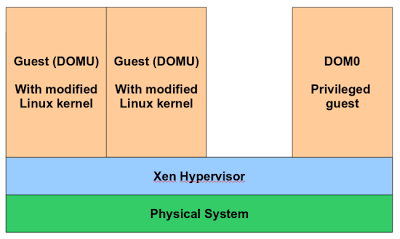
\includegraphics[width=8cm]{bilder/xen.png}
    \caption{Xen Architektur \citep{kvm:002}}
  \end{center}
\end{figure}

Als weitere Gastsysteme lassen sich wie auch bei KVM beliebige unmodifzierte Gastsysteme wie Linux-Distributionen oder Windows-Systeme installieren. Besonders ist aber, dass sich auch Linux-Distributionen mit ebenfalls modifiziertem Kernel laden lassen, die direkter mit dem Hypervisor zusammen arbeiten und so eine höhere Performance bieten.

\subsubsection{Hosted Hypervisors}

Ein Hosted Hypervisor ist ein \ac{VMM}, der als Anwendungsprogramm innerhalb eines Hostbetriebssystems läuft. Es ist somit möglich, auch andere Programme neben dem Hypervisor und seinen Gastbetriebssystemen zu verwenden.

\begin{figure}[!ht]
  \begin{center}
    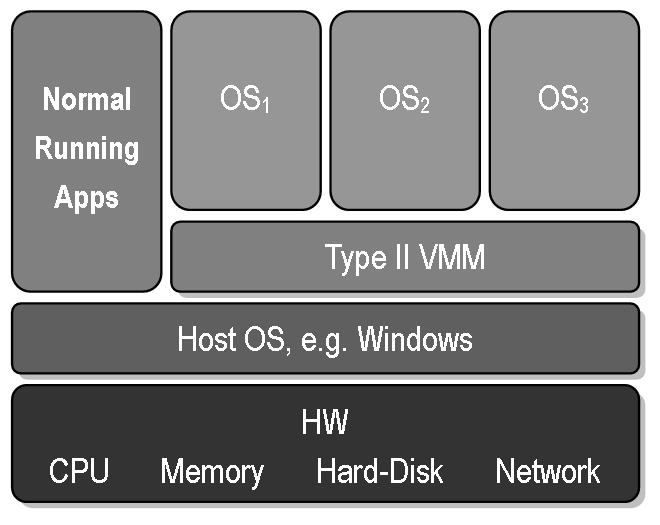
\includegraphics[width=8cm]{bilder/VMM-Type2.jpg}
    \caption{Virtual Machine Monitor Type II \citep{wiki:003}}
  \end{center}
\end{figure}

Größter Vorteil dieser Variante ist es also, dass das Hostsystem auch für gewöhnliche Benutzerarbeiten zur Verfügung steht und nicht ausschließlich zur Virtualisierung verwendet werden muss. Diese Virtualisierungslösung lässt sich sehr einfach nachträglich auf eine Vielzahl von Betriebssystemen installieren und auch wieder deinstallieren. Ein typische Vertreter dieser Hypervisor-Klasse ist zum Beispiel VirtualBox von Oracle \citep{wiki:004}.

\subsubsection{Unikernels}

Eine relativ neue Entwicklung innerhalb der Systemvirtualisierung mittels Hypervisor sind die sogenannten Unikernels. Vertreter dieser Idee kommen zum Beispiel aus dem Bereich der \ac{SOA} oder der Microservice Architecture. In diesen Architekturen wird versucht, die Teile eines IT-Systems als einzelne Dienste zu betrachten, die (meist über Netzwerk) miteinander kommunizieren. Es ist dabei von Vorteil, wenn diese Dienste jeweils eine bestimmte Aufgabe erledigen und über eine einfache Schnittstelle angesprochen werden können. Solche Dienste können nun jeweils über eine eigene \ac{VM} innerhalb der Virtualisierung abgebildet werden. Hierbei wird nun kritisiert, dass die Installation eines kompletten Gastbetriebssystems und die in ihm laufenden Anwendungsprogramme meist wesentlich mehr Resourcen und Programmcode verwenden und mehr Zugriffspunkte bieten, als für den eigentlichen Dienst benötigt wird. Als konzeptionelles Beispiel stellen wir uns hier einmal einen Dienst vor, der als einzige Aufgabe hat, mit Hilfe einer fortlaufenden Zahl neue Kundennummern zu generieren. Es ist nun durchaus nachvollziehbar, dass ein komplettes Gastbetriebssystem inkl. aller in ihm installierten Zubehörprogramme, Dokumentationen und Treiber sehr viel mehr Resourcen verbraucht, als für die eigentliche Operation sinnvoll erscheint. Die höhere Menge an Quellcode und typische Betriebssystemschnittstellen stellen zudem auch ein erhötes Sicherheitsrisiko dar, da sie potentiell mehr Angriffsvektoren bieten. Als Antwort entstehen deshalb in jüngster Vergangenheit neue Lösungen, bei denen man seinen eigentlichen Programmcode mit Hilfe einer Library entwickelt, die einfache Schnittstellen zur Verfügung stellt um z.B. Netzwerkkommunikation o.ä. zu betreiben. Der Programmcode wird dann mit Hilfe dieser Library in eine sehr viel kleinere \ac{VM} kompiliert, die wieder mit Hilfe eines Hypervisors ausgeführt werden kann. Ein Beispiel für eine solche Library ist MirageOS \citep[Vgl.][]{MadMorAnd13}.

\begin{figure}[!ht]
  \begin{center}
    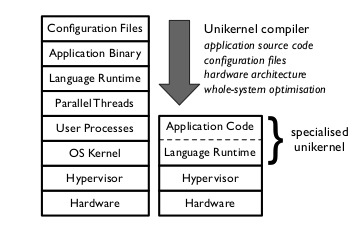
\includegraphics[width=8cm]{bilder/comparison-vm-unikernel.png}
    \caption{Vergleich klassische VM und Unikernel \citep[Abb. 1]{MadMorAnd13}}
  \end{center}
\end{figure}

Ein Nachteil dieser Lösung ist, dass man lediglich Funktionalität wiederverwenden kann, die genau durch die benutzte Library zur Verfügung steht. So kann man auch lediglich in der Programmiersprache arbeiten, die der Compiler der Library versteht. Im Falle von MirageOS ist dies die Sprache Ocaml. Es ist somit zum Beispiel nicht möglich, einen PHP-Interpreter zu starten und PHP-Scripte auszuführen, wie das mit allen gängigen Betriebssystemen wie Linux, MacOS oder Windows der Fall ist. Unikernels lassen sich somit zumindest bisher nur für sehr spezielle Dienste und Problemestellungen einsetzen.

\subsection{Betriebssystemvirtualisierung mittels OS-Containern}
